\documentclass[UTF8]{ctexart}
\usepackage{datetime}
\usepackage{geometry}
\usepackage{array}
\usepackage{graphicx}
\geometry{a4paper,left=1cm,right=2cm,top=1cm,bottom=1cm}
\title{\Huge 电工电子实验中心}
\date{2019 年 10 月 24 日}
\author{\Large 实验报告}

\begin{document}

\maketitle
\vspace{6\baselineskip}
\renewcommand\arraystretch{1.5}
\begin{table}[h]
    \centering
    \Large
    \setlength{\tabcolsep}{5mm}{
        \begin{tabular}{rcrc}
            课程名称: & 数字电子技术 & 实验项目: & 组合逻辑电路 \\

            姓名:     & xxx       & 学号:     & xxxxxxxxx    \\

            班级:     & xxxxxxx      & 日期:     & \date{10.24} \\

            地点:     & 3313         & 成绩:     &              \\
        \end{tabular}}
\end{table}

\vspace{10\baselineskip}

\centering
南京航空航天大学 \\
\newpage
\begin{enumerate}
    \large
    \vspace{1\baselineskip}
    \item[一.]  预习:
          \begin{itemize}
              \item 设计任务:
                    \begin{itemize}
                        \item [1.] 设计三人表决器电路\\
                              要求:
                              \begin{itemize}
                                  \item [1)] 使用1片74LS00。

                              \end{itemize}
                        \item [2.] 设计一位全加器\\
                              要求:
                              \begin{itemize}
                                  \item [1)] 使用1片74LS00及1片74LS86。

                              \end{itemize}
                    \end{itemize}
              \item 原理及设计方案:\\
                    \begin{itemize}
                        \item[1.] 三人表决器电路\\
                              \begin{itemize}
                                  \item 逻辑抽象:\\
                                        用A、B、C分别表示三个人,同意为“1”,不同意
                                        为“0”;Y表示表决结果,通过为“1”,不通过为“0”。三
                                        个人中有任意两个人同意则表决的结果为通过。\\

                                  \item 真值表\\
                                        \setlength{\tabcolsep}{10mm}{
                                            \begin{tabular}{c|c|c|c}
                                                A & B & C & Y \\
                                                \hline
                                                0 & 0 & 0 & 0 \\
                                                0 & 0 & 1 & 0 \\
                                                0 & 1 & 0 & 0 \\
                                                0 & 1 & 1 & 1 \\
                                                1 & 0 & 0 & 0 \\
                                                1 & 0 & 1 & 1 \\
                                                1 & 1 & 0 & 1 \\
                                                1 & 1 & 1 & 1 \\
                                            \end{tabular}}

                                        \vspace{1\baselineskip}
                                  \item 表达式化简\\
                                        \begin{itemize}
                                            \centering
                                            \Large
                                            \item $Y=AB+BC+AC$
                                            \item $Y=B(A+C)+AC$
                                            \item $Y=B\overline{(\bar{A}\bar{C})}+AC$
                                            \item $Y=\overline{\overline{B\overline{\bar{A} \bar{C}}}\cdot \overline{AC}}$
                                        \end{itemize}

                                        \newpage
                                  \item 逻辑图\\
                                        \begin{figure}[h]
                                            \centering
                                            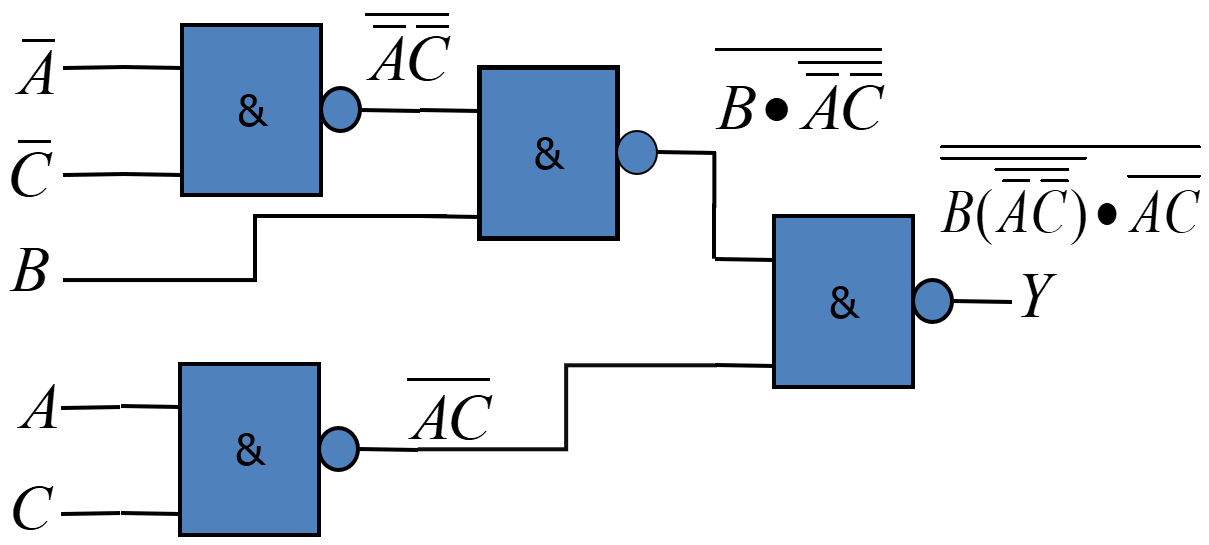
\includegraphics[scale=0.6]{1.png}
                                            \label{fig:label}
                                        \end{figure}

                                  \item 芯片连接\\
                                        \begin{figure}[h]
                                            \centering
                                            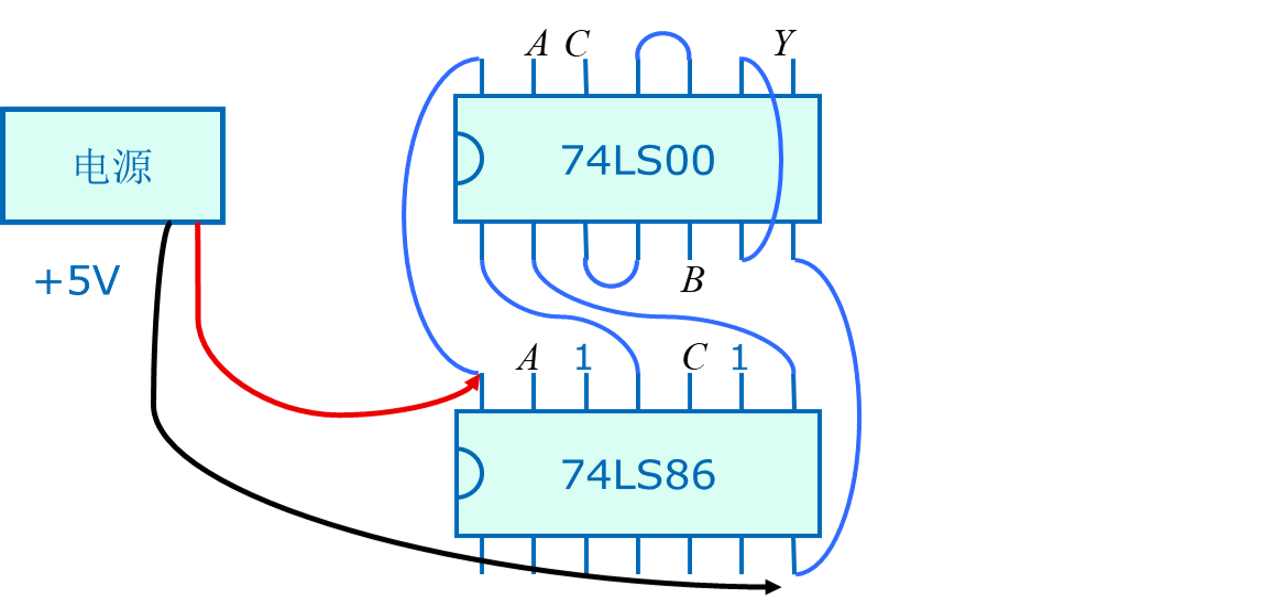
\includegraphics[scale=0.6]{2.png}
                                            \label{fig:label}
                                        \end{figure}
                              \end{itemize}

                        \item[2.] 一位全加器\\
                              \begin{itemize}
                                  \item 设计\\
                                        A、B为要相加的数,Ci为低位来的进位,S为和,Co为进位输出。\\

                                  \item 真值表\\
                                        \setlength{\tabcolsep}{10mm}{
                                            \begin{tabular}{c|c|c|c|c}
                                                A & B & $C_i$ & S & $C_o$ \\
                                                \hline
                                                0 & 0 & 0     & 0 & 0     \\
                                                0 & 0 & 1     & 1 & 0     \\
                                                0 & 1 & 0     & 1 & 0     \\
                                                0 & 1 & 1     & 0 & 1     \\
                                                1 & 0 & 0     & 1 & 0     \\
                                                1 & 0 & 1     & 0 & 1     \\
                                                1 & 1 & 0     & 0 & 1     \\
                                                1 & 1 & 1     & 1 & 1     \\
                                            \end{tabular}}

                                        \vspace{1\baselineskip}

                                        \newpage
                                  \item 表达式化简\\
                                        \begin{itemize}
                                            \centering
                                            \Large
                                            \item $S=A\oplus B\oplus C_i$
                                            \item $C_o=AB+BC+AC$
                                            \item $S=A\oplus B\oplus C_i$
                                            \item $C_o=\overline{\overline{AB}\cdot\overline{(A\oplus B)\cdot C_i}}$
                                        \end{itemize}

                              \end{itemize}
                    \end{itemize}


              \item 计算及仿真:


          \end{itemize}
    \item[二.]  实验目的:
          \begin{itemize}
              \item [1.] 掌握组合逻辑电路设计,安装,调试的基本方法。
              \item [2.] 了解组合逻辑电路设计中最小化(集成芯片数量最少)的概念和实现方法。
              \item [3.] 观察组合逻辑电路中存在的冒险现像。
          \end{itemize}
    \item[三.]  实验仪器与器件:
          \begin{itemize}
              \item 实验仪器:\\
                    \setlength{\tabcolsep}{30mm}{
                        \begin{tabular}{lr}
                            双踪示波器   & 1台 \\
                            信号发生器   & 1台 \\
                            直流稳压电源 & 1台 \\
                            万用表       & 1台 \\
                        \end{tabular}}
              \item 实验器件:\\
                    \setlength{\tabcolsep}{30mm}{
                        \begin{tabular}{lr}
                            74LS00 & 多片 \\
                            74LS20 & 多片 \\
                            74LS86 & 1片  \\
                        \end{tabular}}
          \end{itemize}
    \item[四.]  实验过程及数据分析:
          \begin{itemize}
              \item 三人表决器\\
                    \setlength{\tabcolsep}{10mm}{
                        \begin{tabular}{c|c|c|c|c}
                            A & B & C & Y(电压)) & Y(状态) \\
                            \hline
                            0 & 0 & 0 &          &         \\
                            0 & 0 & 1 &          &         \\
                            0 & 1 & 0 &          &         \\
                            0 & 1 & 1 &          &         \\
                            1 & 0 & 0 &          &         \\
                            1 & 0 & 1 &          &         \\
                            1 & 1 & 0 &          &         \\
                            1 & 1 & 1 &          &         \\
                        \end{tabular}}
              \item 一位加法器\\
                    \setlength{\tabcolsep}{5mm}{
                        \begin{tabular}{c|c|c|c|c|c|c}
                            A & B & $C_i$ & S(电压)) & S(状态) & $C_o$(电压) & $C_o$(状态) \\
                            \hline
                            0 & 0 & 0     &          &         &             &             \\
                            0 & 0 & 1     &          &         &             &             \\
                            0 & 1 & 0     &          &         &             &             \\
                            0 & 1 & 1     &          &         &             &             \\
                            1 & 0 & 0     &          &         &             &             \\
                            1 & 0 & 1     &          &         &             &             \\
                            1 & 1 & 0     &          &         &             &             \\
                            1 & 1 & 1     &          &         &             &             \\
                        \end{tabular}}
          \end{itemize}
\end{enumerate}
\end{document}